\documentclass{ecnreport}

\stud{EMARO2 / ARIA-ROBA}
\topic{Advanced Visual Geometry}

\begin{document}

\inserttitle{Advanced Visual Geometry}

\insertsubtitle{Lab 1: Homography-based visual odometry}


\section{Content of this lab}

The goal of this lab is to perform Augmented Reality (AR) from a sequence of images.\\
The only information that we have is that the camera is observing a mostly planar environment, 
where we want to display the 3D model of a robot (AR), see \Fig{fig:ar} for an overview.

\begin{figure}[h!]
\centering\label{fig:ar}
 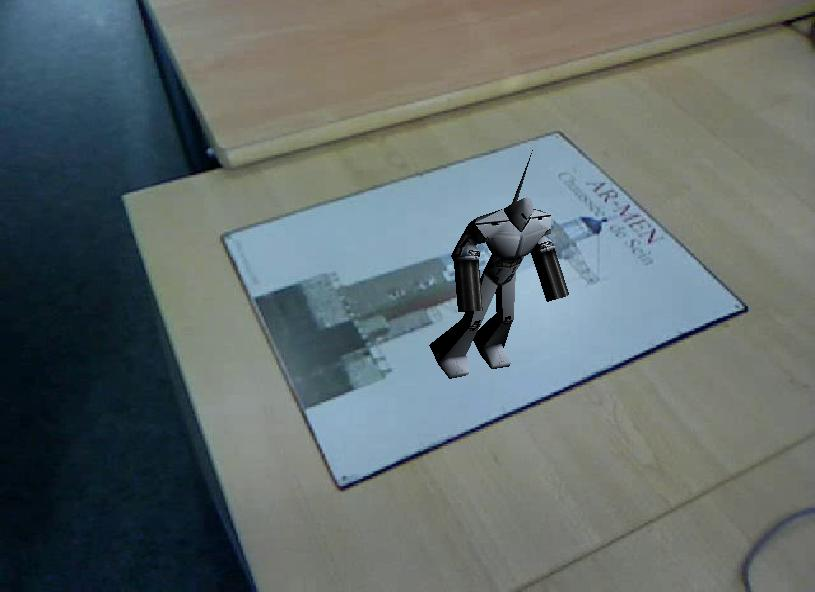
\includegraphics[width=.5\linewidth]{ar}
 \caption{Current image with 3D robot AR display}
\end{figure}

AR needs a 3D transform between the camera and the world frame. By doing homography-based visual odometry (VO), we can do this pose estimation 
with regards to a reference 3D plane. \\
The goal is thus to load the video file, and go through the images with all the necessary steps to perform AR. Two libraries will be used to do so: 
\begin{itemize}
 \item OpenCV 3 to read images from files or camera, perform low-level image processing\footnote{Open source Computer Vision, http://opencv.org}. We use version 3 as it includes
 the homography matrix decomposition. 
 \item ViSP to manipulate 3D points, camera pose and use vectors and matrices\footnote{Visual Servoing Platform, http://visp.inria.fr}
\end{itemize}
The actual classes that are used are detailed in Appendix \ref{sec:classes}.

\subsection{Environment setup and how to compile}

To use this lab you need to initialize the ROS environment (even if the lab is not actually using ROS) in order to have access to the ViSP library, and OpenCV 3 which is not shipped with Ubuntu except from the ROS packages.
To do so, download the following file and execute it:
\begin{center}\cppstyle
\begin{lstlisting}
        wget http://www.irccyn.ec-nantes.fr/~kermorga/files/ros_user_setup.sh
        sh ros_user_setup.sh
\end{lstlisting}
\end{center}

This lab is available on GitHub. The package can be downloaded through git and compiled with the sequence:
\begin{center}\cppstyle
\begin{lstlisting}
 git clone https://github.com/oKermorgant/ecn_visualodom.git
 cd ecn_visualodom
 mkdir build
 cd build
 cmake ..
 make
\end{lstlisting}
\end{center} 

The video should be downloaded from my website in the lab directory:
\begin{center}\cppstyle
\begin{lstlisting}
 wget http://www.irccyn.ec-nantes.fr/~kermorga/files/armen.mp4
\end{lstlisting}
\end{center} 

It may be useful to use an IDE like Qt Creator, to do so you have to launch it from the command line then:
\begin{itemize}
 \item Load the \texttt{CMakeLists.txt} file as a new project
 \item Set the \texttt{build} folder as the build folder
\end{itemize}
 

\subsection{Structure of the \texttt{ecn\_visualodom} folder}

The folder has the classical structure of a C++ project:
\begin{figure}[h]\centering
\begin{minipage}{.05\linewidth} ~ \end{minipage}
\begin{minipage}{.75\linewidth}
 \dirtree{%
.1 ecn\_visualodom. 
.2 include.
.3 ecn\_visualodom. 
.4 ar\_display.h\DTcomment{augmented reality code}.
.4 video\_loop.h\DTcomment{load and read video file}.
.4 visual\_odom.h\DTcomment{VO class header}.
.2 src.
.3 visual\_odom.cpp\DTcomment{VO class to be modified}.
.2 armen.mp4\DTcomment{video file}.
.2 CMakeLists.txt\DTcomment{CMake file}.
.2 vo.cpp\DTcomment{main file to be modified}.
} 
\end{minipage}
%\begin{minipage}{.2\linewidth} ~ \end{minipage}
\caption{Files used by the package}
\end{figure}

The only files to be modified are \texttt{visual\_odom.cpp} that is the visual odometry class and performs visual odometry between two consecutive frames, and \texttt{vo.cpp} that is the main 
C++ file and uses visual odometry to estimate the current pose of the camera with regards to the world frame.


\subsection{Expected work}

The goal is to implement an homography-based visual odometry and test it on the \texttt{armen.mp4} video.
The main steps are already written in the code as comment sections. The \texttt{VisualOdom} class will be doing most of the job, except for the initial pose estimation. 
Dedicated OpenCV of ViSP classes or functions will also do most of the job and the goal of the lab is also to get used to them.

The next section details the homography-based visual odometry algorithm and its most important steps.

\def\n{\mathbf{n}}
\def\t{\mathbf{t}}
\section{Homography-based visual odometry}

The basis of the visual odometry from homography is to compute an homography from two views of the same plane. 
If the equation of the plane is written $\X^T\n = d$ in the first camera frame, then the homography matrix is $\H = \R + \t\n^T/d$
where $(\t, \R)$ express the transform from camera 1 to camera 2 as shown in \Fig{fig:homog}.


\begin{figure}[h!]
\centering\label{fig:homog}
 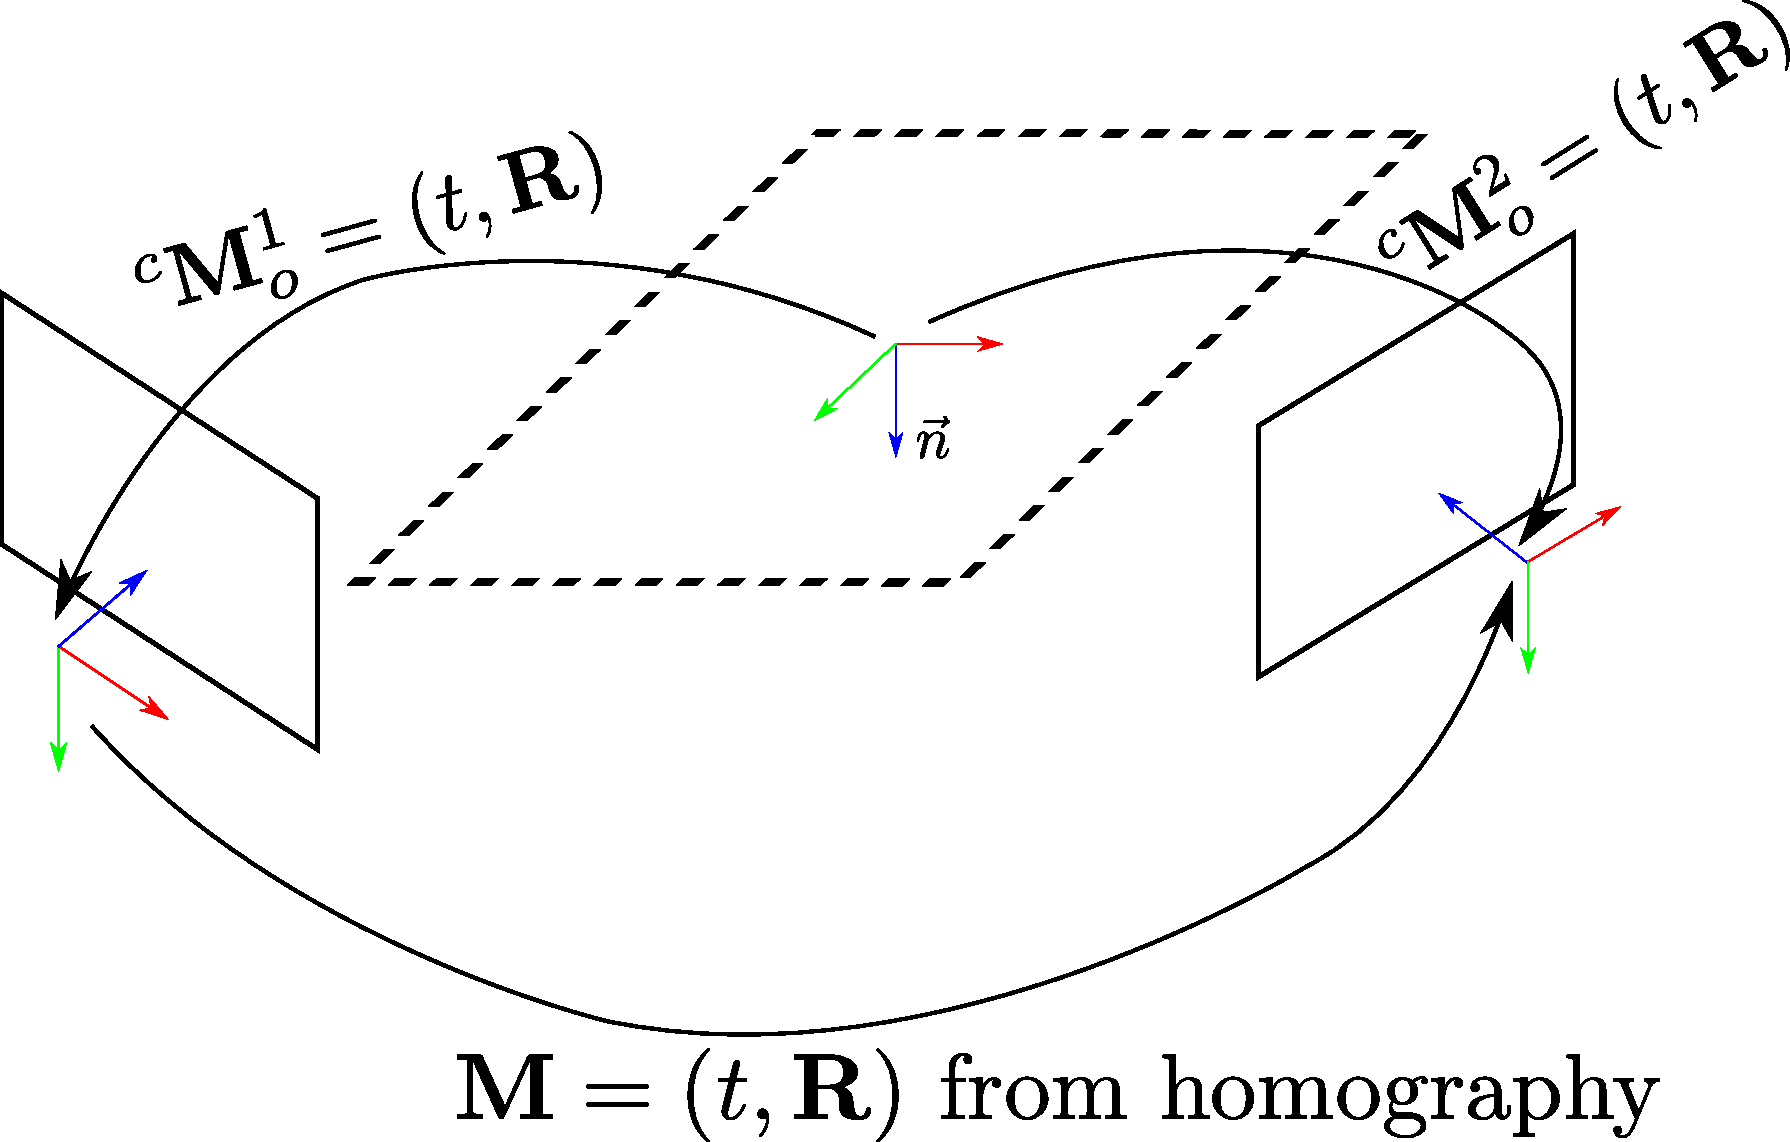
\includegraphics[width=.5\linewidth]{homog}
 \caption{Two views of a given 3D plane links 3 transforms.}
\end{figure}
However, in order to display any 3D model with AR, an initial pose $\cMo$ has to be estimated for the initial camera. We first recall the relative
odometry before giving clues about the initial pose estimation.

\subsection{Relative odometry from homography}

The core algorithm is to compute the relative odometry, that is the transform between the two camera frames. It corresponds to the method \texttt{VisualOdom::process}.
The algorithm to follow is:
\begin{enumerate}
  \item Convert image to gray level
 \item Detect and compute keypoint descriptors in the new image
 \item Match keypoints with the ones from the previous image
 \item With RANSAC, compute homography and also get matches inliners 
 \item Decompose homography to get $(\t,\R,\n)$ candidates\\
  A method in OpenCV
will give us all candidates (usually 4) under the form of 3 vectors of dimension 4: translations, rotations and normal to the plane. Candidates 
are stored under a \texttt{vector} of \texttt{Homography}, a custom structure used to regroup $(\t,\R,\n)$ (see \Sec{sec:homog}).
 \item Prune candidates that give a negative Z for at least 1 point \\ The corresponding loop is already in the code but the condition to consider a candidate to be valid or not has to be defined.
 \item There still may be two candidates, keep the one that has the normal $\n$ closer to the estimated normal
\end{enumerate}
The last step shows that a guess for the normal has to be given in order to find the best candidate homography. This can be done with the \texttt{VisualOdom::setNormalGuess} in the main code (around line 24). In our case we assume
we observe a horizontal plane with a camera also placed horizontally. This is sufficient to have a corse estimate of the normal to the plane in the camera frame.

At the end of the whole sequence, we have a homography decomposition $(\t,\R,\n)$ without the scale factor. Actually OpenCV gives us $\t/d$ as $\t$ as they cannot be separated without
extra information. If we have an estimation of the value $d$, we can easily compute the true translation with $d.\t$. This $d$ estimation is stored in the \texttt{VisualOdom} class as \texttt{d\_guess}.

The final step is to prepare for the next image: the parameters $(d,\n)$ of the plane equation have to be rewritten in the frame of camera 2.
\begin{enumerate}
 \item Updating $\n$ is only a matter of frame change as we have $\R$.
 \item Updating $d$ can be done with only one point, so in practice we compute the new $d$ from all the points and then take the mean value.
\end{enumerate}
We now detail how to get an initial guess for $d$.


\subsection{Initial plane parameter from assumed translation}
\label{sec:init}

The scale factor is given by the size of the 3D model to be displayed. In practice this amounts to fix the initial translation ${}^c\t_o = (-0.1,-0.1,0.7)$.
This translation can be used to have a first estimation of the plane parameter $d$ after the first homography has been computed.
Indeed, in this case we have the normal to the plane and we can just set $d = \n^T{}^c\t_o$. This value can then be used to rescale the relative transform 
that was extracted from the homography. 

\subsection{Overall algorithm}

By combining the relative transform from homography and the initial guess from known translation, after the second image we can have the whole information:
\begin{enumerate}
 \item Get unscaled transform from initial homography, this gives us $(\t,\R)$ between the cameras and the normal $\n$ to the plane in the first camera frame.
 \item Get the rotation matrix corresponding to the Z-axis of the plane aligning with the $\n$ axis of the camera frame (\texttt{VisualOdom::getRotationFromNormal}). 
 \item Build the full transform $\cMo(0)$ for the first image (variable \texttt{cMo0})
  \item Compute the scale factor $d$ from $\n$ and the known translation ${}^c\t_o$ and initialize its value in the visual odometer (\texttt{VisualOdom::setDistance})
  \item Rescale the relative transform $\t \rightarrow d.\t$
\end{enumerate}

After this initialization, the scale factor will be updated at each iteration from the previous value and the current camera pose just has to be updated from the previous one and the relative
transform found by the homography.

In practice, we may experience a scale drift and perform all homographies with regards to the initial image.


\appendix
\section{Main classes and tools}\label{sec:classes}

\subsection{ViSP classes}

This library includes many tools for linear algebra, especially for 3D transformations. 
The documentation is found here: \url{http://visp-doc.inria.fr/doxygen/visp-daily/classes.html}.\\
The main classes from ViSP (at least in this lab) are:
\begin{itemize}
\item \texttt{vpMatrix} represents a classical matrix, can then be transposed, inversed (or pseudo-inversed), multiplied with a vector, etc.
\item \texttt{vpColVector} is a column vector with classical mathematical properties.
\item \texttt{vpHomogeneousMatrix} is a $4\times 4$ 3d transform matrix. They can be multiplied to compose transforms.
\end{itemize}
These class can be declared and used as follows:
\begin{center}\cppstyle
\begin{lstlisting}
       vpMatrix M(2,6); 	// matrix of dim. 2x6
       M[0][0] = M[1][1] = 1;	// element-wise assignment
       vpColVector v(6);	// column vector of dim. 6
       v[0] = 1;		// element-wise assignment
       M*v;			// matrix-vector multiplication
\end{lstlisting}
\end{center}

\subsection{The \texttt{Homography} structure}
\label{sec:homog}

This structure is a simple object that regroups values for $(\t,\R,\n)$. From an instance \texttt{H}, they can be accessed with \texttt{H.t}, 
\texttt{H.R} and \texttt{H.n}. \texttt{t} and \texttt{n} are \texttt{vpColVector} while \texttt{R} is a \texttt{vpRotationMatrix}.

\subsection{The \texttt{VisualOdom} class}

This class does most of the job (at least when you add the correct missing code). It is initialized from the camera parameters and a flag telling if the homography
should be computed relative to the initial image or relative to the previous image (inducing scale drift).\\
The existing methods are:
\begin{itemize}
 \item \texttt{bool process(cv::Mat \&, vpHomogeneousMatrix \&M)} \\ 
 Main method, processes a new image and returns the corresponding transform. Returns True if everything went fine. 
 \item \texttt{void setDistance(double )}: sets the estimated plane parameter $d$
 \item \texttt{void getRotationFromNormal(vpRotationMatrix \&)}: give the rotation matrix between the plane frame and the camera frame. Can only be used
 if at least one homography was computed.
  \item \texttt{void getNormal(vpColVector \&}: get the plane parameter $\n$ computed from the last homography. Useful to compute the initial value $d$ at shown in \Sec{sec:init}.
\end{itemize}

Most of the variables are already defined, the attributes of the class can be read in \texttt{visual\_odom.h}. In particular, 
these useful variables are already available as class attributes:
\begin{itemize}
\item Stored image \texttt{im1}, image that can be used for gray-level conversion \texttt{img}
 \item Keypoints (\texttt{kp1, kp2}) and their descriptors (\texttt{des1, des2})
 \item Keypoint detector and descriptor: \texttt{akaze}
 \item Matcher and matches (\texttt{matcher, matches})
 \item Calibration matrices: \texttt{Kcv} for OpenCV functions, \texttt{K} and \texttt{Ki} (inverse) for ViSP matrix multiplication
 \item Homography matrix (\texttt{Hp}, OpenCV format) and RANSAC mask for inliers (\texttt{mask})
 \item Vector of homography structures \texttt{H} used to analyze the candidates and prune them if needed.
\end{itemize}




\end{document}
